% Full draft for a conference / journal submission — generic template (plain article class). To move to a venue class
% (IEEEtran, acmart, llncs, ...), keep the body and replace the preamble and the front matter.
% Build:  latexmk -pdf main.tex
% Figures: figures/paper_figures.ipynb (style: figures/paper_style.py; dataset_construction.py runs on the server)
% Notes for the authors would be in \todo{...} (red). The previous draft is in _da_cancellare/.
\documentclass[11pt,a4paper]{article}
\usepackage[margin=2.5cm]{geometry}
\usepackage[T1]{fontenc}
\usepackage[utf8]{inputenc}
\usepackage{lmodern}
\usepackage{amsmath,amssymb}
\usepackage{graphicx}
\usepackage{booktabs}
\usepackage{xcolor}
\usepackage{tikz}
\usetikzlibrary{arrows.meta,positioning,shapes.misc}
\usepackage[numbers,sort&compress]{natbib}
\usepackage{xr-hyper}
\usepackage[colorlinks=true,linkcolor=blue!50!black,citecolor=blue!50!black,urlcolor=blue!50!black]{hyperref}
\def\UrlBreaks{\do\/\do-\do\_\do.}
\usepackage{authblk}
\usepackage{orcidlink}
\renewcommand\Affilfont{\small}

\externaldocument[S-]{supplementary}
\newcommand{\todo}[1]{\textcolor{red}{[\textbf{TODO:} #1]}}
\newcommand{\anon}{\operatorname{anon}}

\title{Reading the Source: Predicting the Reliability of Unseen News Publishers from the Anonymized Text
of Their Articles}
\author[1]{John Bianchi\,\orcidlink{0009-0006-2582-1480}\thanks{Corresponding author: John Bianchi
(\texttt{john.bianchi@imtlucca.it}).}}
\author[2]{Manuel Pratelli\,\orcidlink{0000-0002-9978-791X}}
\author[1]{Fabio Pinelli\,\orcidlink{0000-0003-1058-6917}}
\author[2,1]{Marinella Petrocchi\,\orcidlink{0000-0003-0591-877X}}
\affil[1]{IMT School for Advanced Studies Lucca, 55100 Lucca, Italy\\
\texttt{\{john.bianchi, fabio.pinelli\}@imtlucca.it}}
\affil[2]{Institute of Informatics and Telematics, National Research Council (IIT-CNR), 56124 Pisa, Italy\\
\texttt{\{manuel.pratelli, marinella.petrocchi\}@iit.cnr.it}}
\date{}

\begin{document}
\maketitle

\begin{abstract}
Expert organizations rate the reliability of news publishers, but they can review only a limited number of outlets.
Computational methods could extend these ratings, yet they are usually evaluated in settings where a model can recognize
the publisher from its name, its journalists, its links or the sister sites that share its articles. In this work, we
investigate whether the NewsGuard score (0--100) of a publisher never seen in training can be inferred from the text of
its articles once its explicit identifiers are masked. We build a dataset of 25,524 articles from 226 English-language
political outlets, with duplicates removed across outlets and one outlet per owner, and we replace links, e-mail
addresses, the outlet's own name and every outlet and journalist mentioned in the text with placeholders. Under an
outlet-disjoint cross-validation, a ridge regression on the hidden states of the frozen Mistral-Small-24B predicts the
score of unseen outlets with a mean absolute error of 15.8 points, against 17.8 for TF-IDF and 22.1 for the best
constant prediction. With five articles per outlet, its error is already lower than that of TF-IDF with all of them. The
gain is limited to the larger pretrained models: the small encoders we tested do not outperform TF-IDF, frozen or
fine-tuned, and an instruction-tuned model asked directly for the score ranks the outlets about as well as their
political orientation. Training on the same outlets, or on outlets of the same owner with their copies, lowers the error
by 6--12 points, whereas masking the identifiers changes it by less than half a point. At equal NewsGuard score, the
models place left-leaning outlets about 9 points above right-leaning ones. We release the code, the trained models, the
out-of-fold predictions and a local tool that applies the method to new articles.
\end{abstract}

\noindent\textbf{Keywords:} news source reliability; publisher reliability inference; media profiling; anonymization;
large language models; text regression; NewsGuard.

% =====================================================================================================================
\section{Introduction}\label{sec:intro}

In contemporary digital media ecosystems, assessing the reliability of news publishers has become an important means
of limiting the spread of misleading or low-quality information~\cite{Bowman2003,Jemielniak2020}. Professional
organizations such as NewsGuard, the Global Disinformation Index and Media Bias/Fact Check evaluate news outlets
according to journalistic standards, including transparency, editorial accountability, factual accuracy and correction
practices. Despite methodological differences, these systems largely agree and provide a stable foundation for
reliability labeling~\cite{lin2023high,DBLP:conf/icwsm/PratelliP22}. Their assessments are made at the level of the
publisher by trained journalists, so many outlets, especially new and small ones, remain unrated for a long time.

A large body of computational work formulates credibility assessment as an article-level classification
task~\cite{pandolfi2020automatic,Przybyla2021plugin,10.1145/3770077,DBLP:journals/dbsk/AdjiLS26}, while media profiling
predicts the factuality and the bias of a source from its articles and other signals~\cite{baly2018predicting,
baly2020written,nakov2024survey}. When the labels come from publisher-level ratings, two shortcuts can inflate the
results. First, the same publisher may appear in training and test data, and a model then learns the publisher instead
of transferable indicators of reliability~\cite{zhou2021hidden,azizov-etal-2024-safari,verhoeven2025yesterday}. Second,
even when publishers are kept apart, the text carries the identity of its source: the outlet's name in signatures and
boilerplate, the names of its journalists, the links to its own pages and, as we show in Section~\ref{sec:groups},
entire articles copied across networks of sites with the same owner. A model can then recognize an outlet, or one of its
sisters, without reading its text. In previous work we classified articles into the reliability levels of their
publishers~\cite{Bianchi2024SAC}. Here we remove both shortcuts and ask how much of a professional reliability rating
can be recovered from the anonymized text of a publisher that the model has never seen.

The text cannot show a rating directly. Journalists verify NewsGuard's criteria outside the articles, for instance by checking the claims of an outlet against
other sources or reading its \emph{about} pages for the disclosure of ownership and financing. The articles can nonetheless carry traits that go with these practices, such as how claims are
sourced and hedged, how news is separated from opinion, and which topics are covered and in what tone. We look for such traits without trying to identify the publisher.

We address this question as a publisher-level regression problem. Language models predict the score of individual
articles, and the predictions for the articles of a publisher are averaged into its score. To approximate the use of
such a system on unrated outlets, the test outlets are never seen in training, outlets of the same owner never fall on
different sides of a split, duplicated articles are removed across outlets, and every article is anonymized before any
model reads it. Our contributions are fivefold:
\begin{enumerate}
  \item We build a dataset of 25,524 articles from 226 English-language political outlets with NewsGuard scores, using
        simple rules, and show that copied articles almost always link outlets of the same owner and that the largest
        such network (164 sites) would otherwise dominate the least reliable level (Section~\ref{sec:data}).
  \item We anonymize the articles by masking the outlet's own name and, with a zero-shot named-entity recognizer, every
        outlet and journalist they mention (Section~\ref{sec:anon}).
  \item We compare TF-IDF, frozen language models from 0.6 to 24 billion parameters with a linear head, a fine-tuned
        encoder and a zero-shot language model, and find that the large frozen models lower the error of TF-IDF by up
        to 2 points with any number of articles per outlet (Sections~\ref{sec:setup}--\ref{sec:k}).
  \item We measure what each protection of the protocol is worth on the same test outlets: an article-level split, or
        outlets of the same owner with their copies, lowers the error by 6--12 points, while masking the identifiers
        changes it by less than half a point (Section~\ref{sec:ladder}).
  \item We analyze the errors by reliability level and political orientation, and we release the code, the models, the
        predictions and a local tool (Sections~\ref{sec:errors}--\ref{sec:tool}).
\end{enumerate}

% =====================================================================================================================
\section{Related Work}\label{sec:related}

\paragraph{Publisher reliability.} Credibility assessment has long been studied at the level of individual
articles~\cite{pandolfi2020automatic,10.1145/3770077}, but the reputation of the source strongly shapes the perceived
quality of information~\cite{doi:10.1080/07421222.2019.1628921}. Rating systems such as NewsGuard, the Global
Disinformation Index and Media Bias/Fact Check (MBFC) largely agree and are commonly used as ground truth for automated
models~\cite{lin2023high,DBLP:conf/icwsm/PratelliP22}. The reliability of a publisher has been estimated from stylistic
patterns~\cite{przybyla2020capturing}, although style separates hyperpartisan from mainstream outlets better than it
detects fake news~\cite{potthast2018stylometric}; from user interactions, social networks, web graphs and
metadata~\cite{bazmi2023multi,DBLP:conf/ecir/PratelliSP25,DBLP:conf/icwsm/WilliamsCC25,DBLP:journals/jdiq/LongoZCZC25};
and, in media profiling, from articles combined with Wikipedia, social media and audience
signals~\cite{baly2018predicting,baly2020written,nakov2024survey}. Large language models have also been asked to rate
named sources~\cite{yang2023large} or to produce weak credibility labels~\cite{Leite2025}. Asking a model about a named
outlet, however, measures what the model already knows about it, which is why we mask the outlet before any model reads
its articles.

\paragraph{Datasets and generalization.} Datasets with source-level labels include NELA-GT~\cite{gruppi2021nela}, a
Czech dataset with four reliability levels~\cite{bohavcek2022fine} and a standardized version of the BAT
corpus~\cite{DBLP:journals/dbsk/AdjiLS26,batDataset}. Zhou et al.~\cite{zhou2021hidden} showed that models trained on
labels inherited from the sources learn the sources themselves, that random article splits overestimate performance, and
that the accuracy on a test site grows with its similarity to training sites with the same label. Later work confirmed
that performance drops under shifts of domain, time and
publisher~\cite{azizov-etal-2024-safari,burdisso-etal-2024-reliability,verhoeven2025yesterday}. Publisher-disjoint
splits, used for instance in the hyperpartisan task of SemEval-2019~\cite{kiesel2019semeval}, solve part of the problem.
They do not prevent sites of the same network from falling on both sides of a split, and they leave the identifiers in
the text. We handle these two cases with ownership groups, deduplication across outlets and anonymization.

\paragraph{Closest studies.} Table~\ref{tab:related} compares our setting with the studies closest to it, which predict
reliability mainly from the text, with labels given to the sources. All those that test on unseen sources report a large
drop in performance: from 0.91 to 0.65 F1 in Rashkin et al.~\cite{rashkin2017truth}, from 0.94 to 0.86 AUC in Horne et
al.~\cite{horne2019robust}, from 0.998 to 0.796 accuracy for BERT in Przyby{\l}a~\cite{przybyla2020capturing} and from
0.97 to 0.72 AUC in Bozarth and Budak~\cite{bozarth2020toward}. None of them keeps the outlets of the same owner apart,
although outlets often share content~\cite{horne2019spirals} and this sharing is itself a signal of
veracity~\cite{gruppi2021tell}, and only Bozarth and Budak remove the names of the outlets from the text. All of them
predict classes. Continuous degrees of reliability have been estimated from the links between news
sites~\cite{burdisso-etal-2024-reliability} and from the web graph, the text and time together~\cite{kondrup2026credibench},
and the credibility of unnamed domains has been classified from their articles by a large language model with web search
and link signals~\cite{eldifrawi2026temporal}. We predict the score on its full scale from the anonymized text alone,
with all the protections above, and we measure what each of them changes.

\begin{table}[t]
\centering\small
\caption{The closest studies. \emph{Input}: \emph{other} are Wikipedia, Twitter, URL and traffic; \emph{links}: a
separate model on web links. \emph{Unseen sources}: test sources absent from the training data (\emph{in part}: in one
experiment). \emph{Owners apart}: outlets of the same owner never on both sides of the split. \emph{Names masked}:
source identifiers removed from the text (\emph{all}: outlets, journalists, links, e-mail addresses). --: not done or
not reported. The targets are classes per article, except Baly et al.\ and Eldifrawi et al.\ (per source) and this work.}\label{tab:related}
\footnotesize\setlength{\tabcolsep}{3.5pt}
\begin{tabular}{lllllll}
\toprule
study & input & labels & unseen & owners & names & target \\
 & & & sources & apart & masked & \\
\midrule
Rashkin et al.~\cite{rashkin2017truth} & text & source type & yes & -- & -- & 4 classes \\
Baly et al.~\cite{baly2018predicting} & text + other & MBFC & yes & -- & -- & 3 classes \\
Fairbanks et al.~\cite{fairbanks2018credibility} & text; links & MBFC & -- & -- & -- & 2 classes \\
Horne et al.~\cite{horne2019robust} & text & NewsGuard, OpenSources & in part & -- & -- & 2 classes \\
Przyby{\l}a~\cite{przybyla2020capturing} & text & PolitiFact, Pew & in part & -- & -- & 2 classes \\
Bozarth \& Budak~\cite{bozarth2020toward} & text or social & MBFC & in part & -- & outlets & 2 classes \\
Eldifrawi et al.~\cite{eldifrawi2026temporal} & text + search, links & MBFC & in part & -- & -- & 3 classes \\
\midrule
this work & text & NewsGuard & yes & yes & all & score 0--100 \\
\bottomrule
\end{tabular}
\end{table}

\paragraph{Models and anonymization.} Fine-tuned bidirectional encoders~\cite{devlin2019bert,warner2024modernbert} are
the standard choice for text classification and regression. When the independent training units are few, an alternative
is to use a large pretrained model as a frozen feature extractor and to train only a linear model on its
representations, as with embedding models that follow a task instruction~\cite{zhang2025qwen3} or with the intermediate
layers of decoder models, which often give better features than the last one~\cite{skean2025layer}. Standard
anonymization tools target personal data, whereas we need to mask the identity of the publisher, which appears through
the names of outlets and journalists. For this purpose we use GLiNER~\cite{zaratiana2024gliner}, a zero-shot
named-entity recognizer that accepts entity types described in natural language.

% =====================================================================================================================
\section{Problem Definition and Methodology}\label{sec:problem}

\subsection{Problem definition}\label{sec:definition}
Let $A$ be a corpus of news articles, each with a text $t_a$ and a publisher $p(a) \in P$, and let $A_p$ be the articles
of publisher $p$. Each publisher has a reliability score $s(p) \in [0, 100]$ assigned by NewsGuard
(Section~\ref{sec:labels}). Article-level annotations are not available, so every article inherits the score of its
publisher and provides only partial and noisy evidence about it. Each publisher also has a political orientation
$o(p) \in \{\text{left}, \text{right}, \text{none}\}$, taken from the \emph{Orientation} field of its NewsGuard rating and
used only for the post-hoc analysis of Section~\ref{sec:orientation}. Before any model reads it, the text of an article
is anonymized by a function $\anon$ that replaces the identifiers of outlets and journalists with placeholders
(Section~\ref{sec:anon}).

\paragraph{Stage 1: article-level estimation.} A regressor $f$ predicts the score of an article,
$\hat{s}(a) = f(\anon(t_a))$.

\paragraph{Stage 2: publisher-level inference.} The score of a publisher is the mean of the predictions for its
articles, $\hat{s}(p) = \frac{1}{|A_p|} \sum_{a \in A_p} \hat{s}(a)$. Predicting it from a subset of $A_p$ shows how
many articles are needed (Section~\ref{sec:k}).

\paragraph{Disjoint publishers and owners.} Since all the articles of a publisher share its score, a random split of the
articles would let the model see the test labels during training. We therefore split the publishers, so that the
publishers of the training and test data are disjoint,
\begin{equation}\label{eq:disjoint}
P_{\text{train}} \cap P_{\text{test}} = \emptyset .
\end{equation}
This condition is not sufficient when publishers of the same owner publish the same articles under different domains.
We therefore also keep one publisher per ownership group $g(p)$ (Section~\ref{sec:groups}), so that $g(p) \neq g(q)$ for
every $p \in P_{\text{train}}$ and $q \in P_{\text{test}}$, and we remove duplicated articles across all publishers.

\subsection{Evaluation metrics and baselines}\label{sec:metrics}
All the metrics compare $\hat{s}(p)$ with $s(p)$ on the publishers of the test folds. Section~\ref{sec:stage1} computes
the same metrics on articles.

\paragraph{Error.} Our primary metric is the mean absolute error, $\mathrm{MAE} = \frac{1}{|P|} \sum_{p} |\hat{s}(p) -
s(p)|$, in NewsGuard points, since a user of the prediction needs to know how far it is from the rating. We also report
the share of publishers predicted within 20 points of their score, $\frac{1}{|P|} |\{p : |\hat{s}(p) - s(p)| \leq
20\}|$, which tells whether a prediction is roughly right; 20 points is the width of the second NewsGuard level (40--59)
and a fifth of the scale.

\paragraph{Ranking.} A reliability score is also used to rank sources, for instance to decide which unrated outlets a
human rater should review first. As secondary metrics we report Spearman's rank correlation $\rho$ between predicted and
true scores and Kendall's $\tau_b$, which accounts for ties, since the NewsGuard scores of the 226 outlets take only 45
distinct values. Both are insensitive to monotone transformations of the predictions, and therefore to a model that
ranks the outlets correctly but compresses their scores. Supplementary Section~\ref{S-app:measures} adds $R^2$, the root
mean squared error and the area under the ROC curve for telling reliable outlets (score $\geq 60$, the NewsGuard
threshold) from the others.

\paragraph{Baselines.} Three baselines use no text:
\begin{itemize}
  \item \textbf{Training median:} the best constant prediction for the MAE, computed on the training publishers of each
        fold.
  \item \textbf{Training mean:} the best constant for the squared error. Neither constant has any ranking ability.
  \item \textbf{Orientation only:} the mean training score of the publishers with the same political orientation. It
        measures how much of the score could be guessed from the political side alone, which matters because orientation
        and reliability are strongly associated in our data (Figure~\ref{fig:dataset}a).
\end{itemize}

\paragraph{Statistical testing.} Intervals are 95\% percentile bootstrap intervals over
publishers~\cite{efron1979bootstrap}, with 10,000 resamples for the results with all the articles and 2,000 for the
curves by number of articles (Section~\ref{sec:k}). Two models are compared on the same resampled publishers (paired
bootstrap), with a two-sided bootstrap $p$-value. The $p$-values are corrected with the Holm
method~\cite{holm1979simple} within three families of tests: the comparisons of every model with TF-IDF on the four
metrics (24 tests), the curves of each model against TF-IDF (16 tests per model), and the comparisons behind specific
statements of the text (24 tests). A comparison that belongs to two families, such as a model against TF-IDF with all
the articles, is reported from the first. Our primary comparison is the MAE of the large frozen models against TF-IDF. A difference is significant when it
remains so after the correction, at the 5\% level; uncorrected intervals (Section~\ref{sec:ladder}, Supplementary
Section~\ref{S-app:anon}) are stated as such. Systematic errors are studied through the signed error $\hat{s}(p) - s(p)$ per NewsGuard level and per orientation
(Sections~\ref{sec:errors}--\ref{sec:orientation}).

% =====================================================================================================================
\section{Dataset}\label{sec:data}

\subsection{Ground truth: NewsGuard}\label{sec:labels}
The publisher-level score $s: P \rightarrow [0, 100]$ comes from NewsGuard~\cite{newsguard}, a professional media rating
service in which trained journalists evaluate online news outlets. Each outlet is assessed against nine journalistic
criteria, which include whether it repeatedly publishes false content, gathers and presents information responsibly,
regularly corrects errors, handles the difference between news and opinion responsibly, avoids deceptive headlines and
discloses its ownership, financing and content creators. The score is the weighted sum of the criteria met. NewsGuard
also derives five levels from the score, 0--39 ($l_1$), 40--59 ($l_2$), 60--74 ($l_3$), 75--99 ($l_4$) and 100 ($l_5$),
which we use to describe the data and the errors. We use the ratings of 23 October 2026, 76\% of which were last updated
in 2025 or 2026, and keep the outlets whose only NewsGuard topic is \emph{political news or commentary}. The ratings are
licensed to the authors and cannot be redistributed.

NewsGuard has been criticized, mostly by right-leaning outlets and politicians, for rating right-leaning outlets more
severely~\cite{oremus2024newsguard}. Right-leaning sources do score much lower on average, but an analysis of
NewsGuard's data finds no evidence of an inherent bias against them~\cite{luhring2025best}, and its ratings largely agree
with those of other raters~\cite{lin2023high}. We take the ratings as the ground truth of the task without assuming that
they are a neutral measure of quality, and Section~\ref{sec:orientation} examines how the errors of the models depend on
orientation.

\subsection{Collection and cleaning}\label{sec:cleaning}
In October 2026 we collected about 200 recent articles per outlet from the websites of the outlets rated by NewsGuard,
saving the raw HTML of every page. The collector follows feeds, sitemaps and homepage links from the newest articles,
respects robots.txt and makes at most one request per second to each site. Of the 1,293 political outlets sent to the
scraper, 674 returned at least one article; the others were unreachable, blocked automated access or exposed no article
pages. We then built the dataset with the simple rules of Table~\ref{tab:cleaning}. The text is re-extracted from the
saved HTML with trafilatura~\cite{barbaresi2021trafilatura} in precision mode, which keeps the main text and drops
navigation, comments and tables. Articles must be in English (langdetect on the first 400 words, with a fixed seed),
have between 100 and 1,500 words and be published from 2025; the length bounds remove short notices and very long pages
such as transcripts and live blogs. Exact duplicates (the same normalized text) and near duplicates (Jaccard similarity
of word 5-grams of at least 0.5, estimated with MinHash~\cite{broder1997resemblance}) are removed \emph{across all
outlets}, keeping the oldest copy, because removing duplicates within each outlet only would leave the same article in
the training and test folds under two different outlets. Finally, an outlet needs at least 10 articles, and outlets of
the same owner are reduced to the one with the most articles (Section~\ref{sec:groups}).

\begin{table}[t]
\centering
\caption{From the collected pages to the dataset: articles and outlets left after each step.}\label{tab:cleaning}
\begin{tabular}{lrr}
\toprule
step & articles & outlets \\
\midrule
political outlets with at least one article & 86,225 & 674 \\
text extracted from the HTML & 85,303 & 668 \\
English & 67,231 & 577 \\
100--1,500 words & 52,027 & 565 \\
published from 2025 & 40,232 & 531 \\
no exact duplicates & 34,799 & 361 \\
no near duplicates (Jaccard $\geq 0.5$) & 33,694 & 347 \\
at least 10 articles per outlet & 33,443 & 287 \\
one outlet per ownership group & \textbf{25,524} & \textbf{226} \\
\bottomrule
\end{tabular}
\end{table}

\subsection{Ownership groups and shared text}\label{sec:groups}
Many outlets are not independent. Content sharing between news outlets is widespread~\cite{horne2019spirals}, and
networks of sites with the same owner publish the same articles, often under different names. A model trained on one
site of a network could then recognize its sisters in the test set without judging their text. We link two outlets if
NewsGuard registers the same owner for them, after removing legal forms and generic words such as \emph{Inc} or
\emph{Media}, or the same parent domain, directly or through other outlets, and we call the connected sets
\emph{ownership groups}. Ownership is thus as recorded by NewsGuard, which may miss informal ties. The 1,293 political
outlets sent to the scraper form 589 groups, in which 797 outlets have at least one sister. Keeping one outlet per group
would remove 704 of them, which we call the \emph{sister outlets}. Figure~\ref{fig:groups} follows them through the
cleaning. Most disappear with the duplicates (from 263 to 94 at the exact-duplicate step), because the sites of a network
publish the same texts and only the oldest copy is kept. The requirement of 10 articles leaves 61, and keeping one outlet
per group removes these.

\begin{figure}[t]
\centering
\includegraphics[width=\linewidth]{figures/groups.pdf}
\caption{Outlets after each cleaning step (articles in parentheses): one outlet per ownership group (hatched
\texttt{//}) and the other outlets of the same groups (hatched \texttt{\textbackslash\textbackslash}, the \emph{sister}
outlets). Duplicate removal takes away most sisters; the
last rule removes the remaining 61.}\label{fig:groups}
\end{figure}

Figure~\ref{fig:network}a shows why the duplicates are a problem. Before deduplication (531 outlets), 298 outlets share
at least one article, as an exact copy or a near duplicate, with another outlet. Of the 3,280 links between them, 3,212
(98\%) join outlets of the same ownership group, and so do 98\% of the 28,156 shared copies, counted per pair of outlets.
The largest network has 164 sites of a single owner, all rated in the lowest NewsGuard level (0--39), which publish
essentially the same articles. After deduplication none of them has 10 articles of its own, so the network is not in the
dataset. Without these rules, sites of this network would have filled both sides of every fold of a split by outlet, and
a model could have scored its test sites by recognizing the copies of its training sites.

Ownership also counts beyond copied text. After deduplication, 59\% of the 81 outlets that still have a sister (the 61
sister outlets and the 20 outlets kept for their groups) are closer to a sister than to any outlet of another group, by
the TF-IDF similarity of their articles (Figure~\ref{fig:network}b; median similarity 0.73 to the nearest sister and
0.65 to the nearest outlet of another group). Outlets of the same owner usually share the same rating (in 74\% of
the cases in Section~\ref{sec:ladder}). Keeping one outlet per group removes this residual dependence between training
and test outlets, and Section~\ref{sec:ladder} measures what keeping the sister outlets, with their copies, would cost.

\begin{figure}[t]
\centering
\includegraphics[width=\linewidth]{figures/network.pdf}
\caption{Ownership groups and text. (a) Outlets linked by shared articles (exact copies or near duplicates, Jaccard
similarity of word 5-grams $\geq 0.5$) at the step ``published from 2025'', before deduplication; each connected
component is drawn separately and the 233 outlets that share no article are not shown. The three largest ownership
groups on the map have their own marker shape (circle, square, triangle); hollow markers are outlets that are not in
the final dataset. Almost every link joins
outlets of the same group. (b) After deduplication, for the 81 outlets with at least 10 articles that have a sister:
cosine similarity of the mean TF-IDF vector of their articles (links, e-mail addresses and the outlet's own name
removed) to the nearest sister ($y$) and to the nearest outlet of another group ($x$); points above the diagonal are
closer to a sister.}\label{fig:network}
\end{figure}

\subsection{Anonymization}\label{sec:anon}
A model could predict the score by recognizing the outlet through its name, its journalists or its links. The function $\anon$ applies three passes to every title and text, each replacing spans with a placeholder without
rewriting the text:
\begin{enumerate}
  \item links and e-mail addresses become \texttt{[URL]} and \texttt{[EMAIL]} (regular expressions);
  \item the outlet's own name, derived from its domain and written joined or spaced, with or without ``the'', becomes
        \texttt{[OUTLET]}; a name that is also a common English word (e.g.\ \emph{The Week}, \emph{Time}) is replaced only
        when capitalized, unless the outlet itself writes it in lowercase;
  \item GLiNER~\cite{zaratiana2024gliner} (\texttt{gliner\_large-v2.1}, threshold 0.5), with the labels \emph{news
        outlet} and \emph{journalist}, replaces the spans it finds with \texttt{[OUTLET]} and \texttt{[AUTHOR]}. It runs
        on windows of 200 words overlapping by 30, since the recognizer reads at most 384 tokens, and of two
        overlapping spans the one with the higher score is kept. A span is replaced only if it contains a capitalized
        word that is not a pronoun and does not touch a placeholder of passes 1--2, because the recognizer also tags
        pronouns such as \emph{I}, common nouns such as \emph{reporters} and the placeholders themselves.
\end{enumerate}
The third pass masks every outlet and journalist, including those other than the publisher, because citing another
outlet (``according to CNN'') can reveal the position of the publisher among the other outlets, and because the
recognizer cannot tell the publisher's own staff from other journalists. Passes 1--2 are needed because the recognizer
alone leaves the outlet's own name in about one article in four. They replace 17,780 mentions of the outlet's own name,
8,559 links and 398 e-mail addresses; GLiNER replaces 41,278 mentions of news outlets and 33,816 of journalists, in
71.8\% of the articles (of the spans it proposes, 73\% of the outlets and 92\% of the journalists pass the filter).

The name of the publishing outlet appears in 37.8\% of the original articles, in 1.7\% after passes 1--2 and in 1.6\%
after the full anonymization, and the leftovers are mostly names that are also ordinary words. This measure, however,
uses the same name as the masking and cannot see what the masking misses. An independent check with the brand name that
NewsGuard records for each outlet finds it in 2.1\% of the articles, concentrated in 17 outlets whose brand differs from
their domain, for instance think tanks and advocacy organizations named in most of their own articles. Social-media
handles, present in 9.5\% of the articles, and some aliases are not masked either. The models read only the body of the
articles, so the titles, where signatures are most frequent, are not used.

The recognizer touches most articles (other outlets in 54\% and journalists in 45\%), and the own-name rule 24\%
(Supplementary Figure~\ref{S-fig:anonymization}). The density of replacements varies with the score. Links are frequent in the least reliable outlets (1.4 per 1,000 words in the 0--39 band, 0.3 in the 75--100 bands),
while the outlets with a perfect score cite other outlets and name journalists most often (6.8 placeholders per 1,000
words for 0--39 and 8.8 for 100). The placeholders therefore keep a trace of how an outlet writes, such as whether it cites sources and signs its
articles, while hiding which outlet it is. We do not remove writing style, topics or
political stance, since they are the signal we study.

\subsection{The final dataset}\label{sec:final}
The final dataset has 25,524 articles from 226 outlets, with a median of 112 articles per outlet and a range from 10 to
201 (Figure~\ref{fig:dataset}). Scores are skewed towards reliable outlets (median 75): 35 outlets are in the lowest
NewsGuard level, 43 in 40--59, 30 in 60--74, 79 in 75--99 and 39 have the maximum score. The articles have a median of
about 760 tokens and at most about 3,000 for every tokenizer we use, so no article is truncated.

Political orientation is strongly associated with reliability in this population (Figure~\ref{fig:dataset}a). Of the 99
right-leaning outlets, 58 are in the two lowest levels, while 51 of the 68 left-leaning outlets are in the two highest,
and the outlets without an orientation are mostly reliable. This structure belongs to the rated outlets as well as to
our sampling (Supplementary Section~\ref{S-app:selection}). A model could therefore partly predict reliability by
recognizing the political side of an outlet, and Section~\ref{sec:orientation} measures how much of the performance
this explains.

The 226 outlets are not a random sample of the 1,293 rated political outlets (Supplementary
Section~\ref{S-app:selection}; Mann--Whitney $p < 10^{-25}$ for the score and $\chi^2$ $p < 10^{-14}$ for the
orientation). The 619 outlets from which no article could be collected have a mean score of 41, against 69 in the
dataset, and 43\% of them are in the lowest level, since unreliable sites are more often offline, blocked or without
article pages. The removal of exact duplicates takes away 170 outlets, 89\% of them in the lowest level and most of them
sites of the network of 164 copies described above. The dataset therefore under-represents the least reliable outlets,
which are also the hardest to predict (Section~\ref{sec:errors}).

\begin{figure}[t]
\centering
\includegraphics[width=\linewidth]{figures/dataset.pdf}
\caption{The 226 outlets: (a) outlets by political orientation and NewsGuard level (each level has its own hatch);
(b) articles per outlet; (c) NewsGuard score of the outlets in the five folds of the outlet-disjoint split.}\label{fig:dataset}
\end{figure}

% =====================================================================================================================
\section{Experiments}\label{sec:experiments}

\begin{figure}[t]
\centering
\resizebox{\linewidth}{!}{%
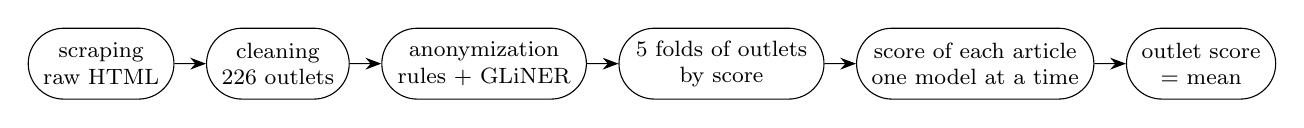
\begin{tikzpicture}[node distance=4mm, box/.style={draw, rounded rectangle, align=center, font=\footnotesize,
  minimum height=9mm, inner sep=3pt}, >={Stealth[length=2mm]}]
\node[box] (s) {scraping\\raw HTML};
\node[box, right=of s] (c) {cleaning\\226 outlets};
\node[box, right=of c] (a) {anonymization\\rules + GLiNER};
\node[box, right=of a] (f) {5 folds of outlets\\by score};
\node[box, right=of f] (m) {score of each article\\one model at a time};
\node[box, right=of m] (o) {outlet score\\= mean};
\foreach \x/\y in {s/c, c/a, a/f, f/m, m/o} \draw[->] (\x) -- (\y);
\end{tikzpicture}}
\caption{The pipeline, from the collected pages to the score of each outlet.}\label{fig:pipeline}
\end{figure}

\subsection{Experimental setup}\label{sec:setup}
Figure~\ref{fig:pipeline} summarizes the pipeline. Following condition~\eqref{eq:disjoint}, we use a 5-fold
cross-validation over outlets, stratified on the exact score: the outlets are sorted by score and, in consecutive blocks
of five, each goes to a different fold at random, so every fold has the same score distribution
(Figure~\ref{fig:dataset}c). Every model is trained on four folds, about 180 outlets and 20,000 articles, and tested on
the fifth, so every outlet is scored once by a model that never saw it. The hyper-parameters of the linear models, the
ridge penalty and, for Mistral-Small-24B, the layer, are chosen by the Spearman correlation per outlet on three inner
folds of the training outlets, built in the same way; those of ModernBERT are fixed. In training every article counts
once, so outlets with more articles weigh more, while in the evaluation every outlet counts once. The models read the
full body of every article, since no article reaches the limit of 4,096 tokens, and do not read the title. We select
models that use the text in different ways, from word counts to large pretrained models used without any adaptation:
\begin{itemize}
  \item \textbf{TF-IDF + ridge.} Word uni- and bi-grams (at most 100,000, with minimum document frequency 5 and sublinear
        term frequency), fitted on the training articles, with a ridge regression~\cite{hoerl1970ridge}. This is the
        standard strong baseline for vocabulary, topic and style.
  \item \textbf{Frozen language models + ridge.} A pretrained model that is not adapted to the task gives one vector per
        article, and a ridge regression on the standardized vectors is the only part learned from our labels.
        \emph{Qwen3-Embedding-8B} and \emph{Qwen3-Embedding-0.6B}~\cite{zhang2025qwen3} are two embedding models of the
        same family. They read the article after the instruction \emph{``Represent this news article to judge the
        reliability and journalistic standards of the outlet that published it''}, and we take the L2-normalized vector
        of the last token (4,096 and 1,024 dimensions). \emph{Mistral-Small-24B}~\cite{mistralsmall} is a base decoder
        model loaded in 4-bit NF4 quantization~\cite{dettmers2023qlora}. We take the mean of the hidden states of an
        intermediate layer~\cite{skean2025layer}, chosen on the inner folds between layer 27 and the last one (40); the
        inner folds choose layer 27 in every fold. \emph{ModernBERT-base} (frozen) is the encoder of the next model
        without any training, represented by the mean of its last hidden states.
  \item \textbf{ModernBERT (fine-tuned).} ModernBERT~\cite{warner2024modernbert} is a bidirectional encoder with 150
        million parameters. We train it end to end on the squared error of $s/100$ with AdamW, learning rate
        $3 \cdot 10^{-5}$, weight decay 0.01, a linear schedule with 6\% warm-up, an effective batch of 32 articles,
        5 epochs, mixed precision and one seed, and keep the model of the last epoch.
  \item \textbf{Mistral-Small-24B-Instruct, zero-shot.} To test whether a language model can rate the articles without
        training, we ask the instruction-tuned version of Mistral for the score of the website that published each
        article, with a prompt that describes the nine NewsGuard criteria and the placeholders (Supplementary
        Section~\ref{S-app:prompt}). Decoding is greedy, the first integer of the answer is the prediction, and the 24
        answers without a number get the mean training score.
\end{itemize}
The two Qwen3 models differ in size and vector dimension, the two ModernBERT models only in their training, and the
frozen and the instruction-tuned Mistral in their weights and in how they use the text.

The ridge penalty is chosen from $\{10^{-3}, \ldots, 1\}$ for TF-IDF and from $\{10, \ldots, 10^6\}$ for the frozen
vectors. The two small frozen models often choose the lowest value, but extending the grid to 0.01 changes their $\rho$
by less than 0.001. All random choices are seeded, and the predictions and the model of every fold are saved, so every
result can be recomputed. On one NVIDIA V100 (32 GB), the frozen vectors take about 2 hours for Qwen3-Embedding-8B and 5
for Mistral-Small-24B, fine-tuning ModernBERT takes 1.5 hours per fold, and each ridge regression takes a few seconds.

\subsection{Stage 1: article-level score estimation}\label{sec:stage1}
We first evaluate the article-level regressors, the intermediate components of the framework, by comparing each test
article with the score of its outlet (Table~\ref{tab:article}). All models rank the articles better than chance.
Mistral-Small-24B is the best, with an error of 17.8 points and a Spearman correlation of 0.61 with the scores of the
outlets. The errors are large: a single article is predicted within 20 points of the score of its outlet in 54--64\% of
the cases with the trained models, against 50\% without text, and the zero-shot model does worse than no text on this
measure (44\%). This is expected, because every article inherits the score of its outlet while individual articles
deviate from the profile of the outlet, as when a reliable outlet publishes a short opinion piece or an unreliable one a
factual report.

\begin{table}[t]
\centering
\caption{Stage 1: articles. Each test article (25,524) is compared with the score of its outlet. The outlet-level
results are in Table~\ref{tab:main}.}\label{tab:article}
\begin{tabular}{lccc}
\toprule
model & MAE (points) & Spearman $\rho$ & within 20 (\%) \\
\midrule
no text (training mean) & 23.0 & -- & 50.4 \\
Mistral-Small-24B-Instruct, zero-shot & 24.3 & 0.233 & 43.8 \\
\midrule
TF-IDF + ridge & 20.4 & 0.429 & 56.6 \\
ModernBERT (fine-tuned) & 20.4 & 0.458 & 58.0 \\
ModernBERT (frozen) + ridge & 20.9 & 0.403 & 55.0 \\
Qwen3-Embedding-0.6B (frozen) + ridge & 21.3 & 0.368 & 54.1 \\
Qwen3-Embedding-8B (frozen) + ridge & 19.4 & 0.525 & 59.3 \\
Mistral-Small-24B (frozen) + ridge & \textbf{17.8} & \textbf{0.614} & \textbf{63.5} \\
\bottomrule
\end{tabular}
\end{table}

\subsection{Stage 2: publisher-level score inference}\label{sec:stage2}
Publisher-level inference is the primary objective of this work. Table~\ref{tab:main} reports the results per outlet
with all the articles, and Figure~\ref{fig:scatter} plots the predicted against the NewsGuard score of every outlet.
Aggregation improves every model. From one article per outlet to all of them, the error of every
trained model falls by 1.5--3.1 points, and the Spearman correlation per outlet rises from 0.62 to 0.735 for
Mistral-Small-24B and from 0.39 to 0.674 for TF-IDF, all significantly. Reliability emerges more clearly from
the articles of a publisher taken together than from any single article.

\begin{table}[t]
\centering
\caption{Stage 2: predicting the NewsGuard score of unseen outlets (226 outlets, all articles). 95\% bootstrap
intervals in brackets (10,000 resamples of the outlets); $^\ast$: significantly better than TF-IDF (paired bootstrap,
Holm correction over the 24 comparisons with TF-IDF). Best value in bold.}\label{tab:main}
\resizebox{\linewidth}{!}{%
\begin{tabular}{lcccc}
\toprule
model & MAE (points) & Spearman $\rho$ & Kendall $\tau_b$ & within 20 (\%) \\
\midrule
no text (training mean) & 22.6 [20.7, 24.5] & $-$0.015 [$-$0.15, 0.11] & $-$0.012 [$-$0.11, 0.09] & 50.9 [44.2, 57.5] \\
no text (training median) & 22.1 [19.9, 24.4] & -- & -- & 54.0 [47.3, 60.6] \\
orientation only (training mean per orientation) & 18.5 [16.7, 20.5] & 0.362 [0.24, 0.48] & 0.260 [0.17, 0.35] & 64.2 [58.0, 70.4] \\
Mistral-Small-24B-Instruct, zero-shot & 24.4 [22.5, 26.2] & 0.348 [0.22, 0.46] & 0.246 [0.16, 0.33] & 41.6 [35.4, 48.2] \\
\midrule
TF-IDF + ridge & 17.8 [16.2, 19.6] & 0.674 [0.60, 0.73] & 0.480 [0.42, 0.54] & 61.5 [54.9, 67.7] \\
ModernBERT (fine-tuned) & 17.5 [15.8, 19.3] & 0.610 [0.52, 0.68] & 0.435 [0.37, 0.50] & 63.7 [57.5, 69.9] \\
ModernBERT (frozen) + ridge & 18.3 [16.6, 20.0] & 0.619 [0.53, 0.69] & 0.446 [0.38, 0.51] & 58.8 [52.7, 65.5] \\
Qwen3-Embedding-0.6B (frozen) + ridge & 18.8 [17.1, 20.6] & 0.626 [0.55, 0.69] & 0.439 [0.38, 0.50] & 57.1 [50.4, 63.7] \\
Qwen3-Embedding-8B (frozen) + ridge & 16.3$^\ast$ [14.8, 17.9] & 0.711 [0.65, 0.76] & 0.514 [0.46, 0.57] & \textbf{69.9}$^\ast$ [63.7, 75.7] \\
Mistral-Small-24B (frozen) + ridge & \textbf{15.8}$^\ast$ [14.3, 17.4] & \textbf{0.735} [0.67, 0.78] & \textbf{0.540} [0.48, 0.59] & 68.1 [61.9, 74.3] \\
\bottomrule
\end{tabular}}
\end{table}

\begin{figure}[t]
\centering
\includegraphics[width=\linewidth]{figures/scatter.pdf}
\caption{Predicted against NewsGuard score, one point per outlet (mean of the predictions for its articles); the
marker shape gives the NewsGuard level; the dashed line is the perfect prediction.}\label{fig:scatter}
\end{figure}

\paragraph{Large frozen models.} Mistral-Small-24B predicts the score of unseen outlets with an error of 15.8 points,
against 22.1 for the best constant, and ranks them with $\rho = 0.735$. Its error is significantly lower than that of
TF-IDF, by 2.0 points [$-2.9$, $-1.2$]. Its ranking ($\Delta\rho = +0.060$ [0.020, 0.104]) and its share of outlets
within 20 points ($+6.6$) are also higher, but these two differences are not significant after the correction for
multiple comparisons (Holm $p = 0.07$ and $0.18$). Qwen3-Embedding-8B significantly lowers the error ($-1.5$ [$-2.3$,
$-0.7$]) and raises the share within 20 points ($+8.4$), while its rank correlation is not significantly higher
($+0.037$). The two large models are not significantly different from each other.

\paragraph{Model size.} The gain comes with the larger models. The 8-billion-parameter Qwen3 model has an error 2.5
points lower than the 0.6-billion one ([$-3.2$, $-1.7$]) and a higher ranking ($+0.085$ [0.039, 0.136]), both
significantly, while the small one is no better than TF-IDF; the two models also differ in the dimension of their
vectors (4,096 against 1,024). Mistral-Small-24B is not significantly better than Qwen3-Embedding-8B, and the frozen
ModernBERT, with 150 million parameters, is not worse than Qwen3-Embedding-0.6B. The evidence concerns small against large models and does not show a steady gain with size. Fine-tuning the small encoder does not close the gap.
The fine-tuned and the frozen ModernBERT cannot be distinguished ($\rho$ 0.610 and 0.619, MAE 17.5 and 18.3), and
neither is better than TF-IDF. The fine-tuned model fits its training articles far better than the test articles (training loss $0.0019$ on $s/100$,
about 4 points of error, against 20.4 on the test articles), yet the frozen version, which cannot memorize the training
outlets, is not better. With fixed hyper-parameters and one seed, this result concerns this small encoder only.

\paragraph{Zero-shot.} Asked directly for the score, the instruction-tuned Mistral ranks the outlets with
$\rho = 0.35$, about as well as the orientation alone, and the error of its raw answers (24.4 points) is larger than
that of a constant. 85\% of its answers are either 65 or 45, so the answer says little more than whether an article
looks reliable. The same model family read through a linear head trained on our labels is instead the best model of the
study ($+0.39$ in $\rho$ and $-8.6$ points of error), in line with other estimation tasks in which a linear head on
hidden states outperforms the text answers of language models~\cite{buckmann2025revealing}.

\paragraph{Orientation.} Predicting the mean training score of the orientation of the outlet gives $\rho = 0.36$ and an
error of 18.5 points, and every trained model ranks the outlets far better. Section~\ref{sec:orientation} shows that the
models also rank outlets within the same orientation.

\paragraph{Compression and other splits.} Every model predicts scores in a narrower range than the true ones
(Mistral-Small-24B between 37 and 96, Figure~\ref{fig:scatter}), so the extremes of the scale are rarely reached
(Section~\ref{sec:errors}) and part of the MAE comes from this compression. Re-mapping the outlet scores with a straight
line fitted inside the training folds lowers every error by 1--3 points, to 14.7 for Mistral-Small-24B, 16.2 for TF-IDF
and 21.2 for the zero-shot model, which then falls below the constant. Mistral-Small-24B remains better than TF-IDF after
this recalibration ($-1.5$ [$-2.7$, $-0.4$]), while the advantage of Qwen3-Embedding-8B is no longer significant
(Supplementary Section~\ref{S-app:robust}). With four more splits made in the same way, the ranking of the models is the
same in every split, and Mistral-Small-24B lowers the error of TF-IDF by 2.0--2.3 points in each of them (Supplementary
Section~\ref{S-app:splits}).

\subsection{How many articles are needed}\label{sec:k}
A practical question for deployment is how many articles of an outlet must be collected. We predict the score of each
outlet from $k = 1, 2, 3, 5, 10, 20, 50$ of its articles, drawn at random, with 20 draws per $k$ and outlet and the same
draws for every model (outlets with fewer than $k$ articles use all of them). Mistral-Small-24B is significantly better
than TF-IDF for every $k$ from 1 to 50, on both the error and the ranking (Figure~\ref{fig:curves}; Holm correction over
the 16 comparisons of each model; for all the articles see Table~\ref{tab:main}). With a single article per outlet its
error is 17.3 points, against 20.5 for TF-IDF, and $\rho = 0.62$, against 0.39. With five articles its error (16.1
points) is already significantly lower than that of TF-IDF with all of them (17.8; $-1.7$ [$-2.6$, $-0.9$]), and its
ranking with five articles (0.71) is also higher than that of TF-IDF with all of them (0.67), although not
significantly. Qwen3-Embedding-8B is significantly better than TF-IDF on the error for every $k$ and on the ranking up to
ten articles. ModernBERT and the two small frozen models are never significantly better than TF-IDF, and
Qwen3-Embedding-0.6B has a significantly larger error from two articles on. All curves flatten after about ten
articles. The advantage of Mistral-Small-24B on both metrics, and of Qwen3-Embedding-8B in ranking, is largest when few
articles are available, as for a new or small outlet.

\begin{figure}[t]
\centering
\includegraphics[width=\linewidth]{figures/curves.pdf}
\caption{Spearman correlation and MAE per outlet as a function of the number of articles read per outlet (mean of 20
random draws per outlet; each model has its own marker and dash pattern); the dashed line is the no-text
baseline.}\label{fig:curves}
\end{figure}

\subsection{Effect of the evaluation protocol}\label{sec:ladder}
Our protocol removes three ways in which a model could recognize an outlet instead of reading its text: the same outlet
in the training data, outlets of the same owner in the training data, and identifiers in the text. To measure what each
protection is worth, we retrain the three ridge models under weaker protocols and test them on the same 25,524
articles of the 226 outlets, in the same folds (Table~\ref{tab:ladder}):
\begin{itemize}
  \item \textbf{Article split:} the folds are drawn over articles, so every test outlet also has articles in the
        training data.
  \item \textbf{Sisters:} the training data of every fold also contains the 89 outlets of the same owners that
        deduplication or the last cleaning rule removed (with at least 10 articles from 2025), with all their articles,
        so the 31 outlets of their groups are tested with a sister in the training data.
  \item \textbf{Original text:} no anonymization.
  \item \textbf{Rules only:} only passes 1--2 of Section~\ref{sec:anon}.
\end{itemize}
Each protocol is compared with the one that differs from it only in the protection removed, that is the sisters with the
original text and the others with the full protocol.

\begin{table}[t]
\centering
\caption{How much each protection matters. MAE and Spearman $\rho$ per outlet on the same test articles and folds; in
parentheses the difference from the protocol that differs only in the protection removed (the original text for the sisters, the full protocol for the others); $^\dagger$: 95\% bootstrap interval of the difference excluding zero.}\label{tab:ladder}
\resizebox{\linewidth}{!}{%
\begin{tabular}{llcccccc}
\toprule
& & \multicolumn{2}{c}{TF-IDF} & \multicolumn{2}{c}{Qwen3-Embedding-8B} & \multicolumn{2}{c}{Mistral-Small-24B} \\
\cmidrule(lr){3-4}\cmidrule(lr){5-6}\cmidrule(lr){7-8}
outlets & protocol & MAE & $\rho$ & MAE & $\rho$ & MAE & $\rho$ \\
\midrule
all 226 & article split & 10.4 ($-$7.4)$^\dagger$ & 0.904 (+0.230)$^\dagger$ & 10.7 ($-$5.6)$^\dagger$ & 0.884 (+0.173)$^\dagger$ & 8.7 ($-$7.1)$^\dagger$ & 0.924 (+0.189)$^\dagger$ \\
 & sisters & 17.1 ($-$0.8) & 0.712 (+0.039)$^\dagger$ & 15.7 ($-$0.3) & 0.733 (+0.009) & 14.9 ($-$0.8) & 0.732 ($-$0.002) \\
 & original text & 18.0 (+0.1) & 0.673 ($-$0.001) & 16.0 ($-$0.3) & 0.724 (+0.013) & 15.7 ($-$0.1) & 0.734 ($-$0.001) \\
 & rules only & 17.7 ($-$0.1) & 0.679 (+0.005) & 15.9 ($-$0.4)$^\dagger$ & 0.724 (+0.013) & 15.7 ($-$0.1) & 0.734 ($-$0.001) \\
 & full protocol & 17.8 & 0.674 & 16.3 & 0.711 & 15.8 & 0.735 \\
\midrule
31 with a sister & sisters & 8.3 ($-$11.6)$^\dagger$ & 0.918 (+0.254)$^\dagger$ & 11.6 ($-$6.9)$^\dagger$ & 0.908 (+0.227)$^\dagger$ & 9.7 ($-$8.7)$^\dagger$ & 0.943 (+0.212)$^\dagger$ \\
 & original text & 19.9 & 0.664 & 18.4 & 0.681 & 18.3 & 0.732 \\
\midrule
195 without & sisters & 18.5 (+0.9)$^\dagger$ & 0.676 (+0.009) & 16.3 (+0.7)$^\dagger$ & 0.707 ($-$0.027) & 15.8 (+0.4) & 0.698 ($-$0.041)$^\dagger$ \\
 & original text & 17.7 & 0.667 & 15.6 & 0.734 & 15.3 & 0.739 \\
\bottomrule
\end{tabular}}
\end{table}

\paragraph{Same outlet.} Separating the outlets has the largest effect. With an article-level split the error falls by
5.6--7.4 points and $\rho$ rises to 0.88--0.92, because the models recognize outlets they have already seen. Under this
split the advantage of Qwen3-Embedding-8B over TF-IDF, which can memorize the vocabulary of each outlet, disappears (MAE
10.7 against 10.4).

\paragraph{Same owner.} Sister outlets in training have almost the same effect on the outlets of their groups. Over the 226
outlets, the sisters change the error by less than one point, because only 31 outlets have one. On those 31 outlets the
error falls by 7--12 points, to 8.3, 11.6 and 9.7 for TF-IDF, Qwen3-Embedding-8B and Mistral-Small-24B, about as low as
with the article-level split on the same outlets (11.7, 12.8 and 9.6). The other 195 outlets do not improve, so the gain
does not come from the larger amount of training data. Since half of the test articles of these 31 outlets have a near
copy among the articles of their sisters, this protocol measures copies and ownership together.

The gain goes with the similarity between training and test texts, as Zhou et al.~\cite{zhou2021hidden} found for sites
with the same label. For the outlets with a sister, adding the sisters raises the cosine similarity (TF-IDF) between a
test article and its most similar training article from 0.19 to 0.60 on average, against 0.16 to 0.18 for the other
outlets, and the larger this increase, the larger the fall of the error. Over the 31 outlets, the Spearman correlation
between the two is 0.60 [0.30, 0.80] for TF-IDF, and 0.25 and 0.32 for the language models, which are not significant
and whose notion of similarity is probably not lexical. Similar texts help because sisters share their ratings: 23 of
the 31 outlets have the same NewsGuard score as all their sisters, and the mean absolute difference between an outlet
and its sisters is 3.8 points, against 29.6 between two outlets of these groups taken at random.

\paragraph{Identifiers.} Anonymization changes the results little. Without any anonymization the error differs from that
of the full protocol by at most 0.3 points, and with the rules alone by at most 0.4, with an uncorrected interval that
excludes zero only for Qwen3-Embedding-8B. No $\rho$ changes significantly, and leaving out the 16 outlets whose brand
name of two or more words is still in their text changes the advantage of Mistral-Small-24B over TF-IDF from 2.0 to 1.8
points. The models therefore do not rely on the identifiers we mask, nor mainly on what they may know about an outlet
from their pretraining. From the frozen vector of the domain name alone, with the same ridge and folds,
Mistral-Small-24B and Qwen3-Embedding-8B rank the outlets with $\rho = 0.39$ and 0.35 (MAE 20.4 and 21.7), about as well
as the orientation alone and far below what they reach from the text (Supplementary Section~\ref{S-app:robust}). An
earlier rule-based anonymization, run through the whole pipeline, leads to the same conclusion (Supplementary
Section~\ref{S-app:anon}).

\paragraph{Boilerplate.} Anonymization leaves in the text the lines that an outlet repeats in many of its articles, such
as invitations to subscribe to a newsletter, donation appeals and disclaimers, and these lines could also let a model
recognize the outlet. We call boilerplate a line that appears in at least three articles and in at least 5\% of the
articles of the same outlet. These lines are 3.0\% of the words and appear in about half of the articles. TF-IDF
retrained without them has an MAE of 17.5, against 17.8 with them. For the language models we borrow the idea of the
explanation methods, which attribute a prediction to the parts of the input~\cite{kozik2024explainability}.
Mistral-Small-24B predicts with a linear function of the mean of its token states, so its prediction splits exactly
into one contribution per token. On 300 articles with boilerplate, these lines contribute 1.9 points on average to a
prediction whose standard deviation is 17.5 points. Removing them from 1,000 such articles, without retraining, moves
the predictions of Mistral-Small-24B, TF-IDF and Qwen3-Embedding-8B by 2.0, 3.3 and 4.8 points on average
(Supplementary Section~\ref{S-app:reading}). The models use the boilerplate a little, but their predictions come mostly
from the body of the articles.

\subsection{Errors by reliability level}\label{sec:errors}
Figure~\ref{fig:errors}a reports the mean signed error per NewsGuard level. Two patterns are common to all models. The
first is a regression towards the centre of the scale. The least reliable outlets are overestimated, with a mean signed
error of $+31$ points for Mistral-Small-24B and $+36$ for TF-IDF in the 0--39 band, the outlets with a perfect score are
underestimated ($-19$ and $-25$), and the outlets in the middle of the scale (60--74) are predicted almost without bias
($-3$ and $-2$). For the trained models the signed error decreases with the true score with a slope between $-0.63$
(Mistral-Small-24B) and $-0.81$ (Qwen3-Embedding-0.6B), so one point of NewsGuard score moves their prediction by only
0.19--0.37 points on average, and that of the zero-shot model by 0.09.

The second pattern is that the extremes are the hardest to predict. With Mistral-Small-24B the error is 31 points in
the 0--39 band and 19 for score 100, against 9 in the 60--74 band. Part of this is a property of the target. The
extremes are reached through criteria that are hardly visible in a single article, such as the repeated publication of
false content or the disclosure of ownership and financing, and the ridge regression shrinks towards the mean when the
text does not separate them. The compression also comes from training on single articles. The slope of the prediction on
the true score is the same per article and per outlet (about 0.37 for Mistral-Small-24B), so the aggregation keeps it. Since the direction of the errors is the same for all models, we
attribute it to our design, a regressor trained on single articles whose scores are then averaged, more than to a
specific architecture; the larger models compress less.

\begin{figure}[t]
\centering
\includegraphics[width=\linewidth]{figures/errors.pdf}
\caption{Where the models err (one bar per model, each with its own hatch). (a) Mean signed error (predicted minus
true score) per NewsGuard level; positive values are overestimates. (b) Mean signed error per political orientation at equal NewsGuard
score (residuals of a linear regression of the signed error on the true score). (c) Spearman correlation within the
outlets of one orientation, with 95\% bootstrap intervals.}\label{fig:errors}
\end{figure}

\subsection{Influence of political orientation}\label{sec:orientation}
Orientation and reliability are associated in our data, with a mean score of 80 for the left-leaning outlets and for
those without orientation and of 54 for the right-leaning ones (Figure~\ref{fig:dataset}a), so we examine whether the
models treat the orientations equally.

\paragraph{Ranking within an orientation.} A model that only recognized the political side of an outlet could not rank
outlets of the same orientation, but all models do (Figure~\ref{fig:errors}c). Mistral-Small-24B reaches $\rho = 0.62$
[0.44, 0.75] within the 99 right-leaning outlets, 0.63 [0.44, 0.78] within the 59 outlets without orientation and 0.38
[0.15, 0.57] within the 68 left-leaning ones, whose scores are concentrated in the two highest levels. TF-IDF and
ModernBERT are lower in every group.

\paragraph{Errors at equal score.} The raw signed errors differ by orientation (Kruskal--Wallis $p < 0.001$ for every
model), mostly because the right-leaning outlets are more often in the low levels, which are overestimated. At equal
NewsGuard score, measured by the residuals of the signed error after removing its linear dependence on the true score
(Figure~\ref{fig:errors}b), a gap remains. With Mistral-Small-24B, left-leaning outlets are predicted $+5.2$ points and
right-leaning ones $-4.3$, a gap of 9.6 points [6.7, 12.3], which becomes 8.8 with a spline of the score and 8.7 with the
level as a fixed effect. The gap is present in the other trained models (4.5--8.4 points) but not in the zero-shot model
(0.1).

This gap is not a mechanical effect of the compression, since shrinking every outlet towards the overall mean produces
no gap at all. It appears when the predictions carry information correlated with orientation beyond the true score, as
when a model that is uncertain about an outlet moves it towards the outlets that write like it, which tend to share its
orientation. A predictor that shrinks each outlet towards the mean of its own orientation, with the slope of
Mistral-Small-24B, would have a gap of 12.6 points [9.9, 14.6]. The models lie between this value and zero: they partly fall back on signals correlated with orientation.

\paragraph{Calibration.} At equal \emph{prediction}, the true scores of left- and right-leaning outlets differ by 0.8
points [$-7.5$, 8.9] for Mistral-Small-24B, 4.8 for Qwen3-Embedding-8B and 7.1 for TF-IDF. None of these differences is
significant, but the intervals are wide, so we can only say that we find no evidence of miscalibration. The difference
is significant for the fine-tuned ModernBERT (12.8), the small frozen models and the zero-shot model (24.8). A predictor
calibrated within groups cannot in general also have equal errors at equal score when the groups have different
means~\cite{kleinberg2017inherent,chouldechova2017fair}. A deployed system would therefore give right-leaning outlets
predictions about 9 points lower than left-leaning ones with the same score, and this must be taken into account when the
predictions are used to prioritize human review.

% =====================================================================================================================
\section{Released Resources and Demonstration Tool}\label{sec:tool}
We release in two repositories everything needed to reproduce and use the study (Supplementary
Section~\ref{S-app:tool} and Supplementary Table~\ref{S-tab:release}). The first contains the pipeline of
Sections~\ref{sec:data}--\ref{sec:experiments} and the code of every table and figure
(\url{https://github.com/bianchi-john/PublisherClassification}). The second contains the four main models of
Table~\ref{tab:main} (TF-IDF, Qwen3-Embedding-8B, Mistral-Small-24B and the fine-tuned ModernBERT) in their five fold
versions, the out-of-fold predictions for every article and the split of the outlets
(\url{https://github.com/bianchi-john/publisher-evaluation}\todo{publish the tool repository and check the link}). The
NewsGuard scores and levels are licensed and are not included in any released file. The text of the articles is not
redistributed either, only their URLs, from which the articles can be collected again and passed through the released
pipeline.

The second repository also contains \emph{Publisher Evaluation}, a tool that runs on the user's machine and applies the
method to new articles. It extracts and checks the text as in Section~\ref{sec:cleaning}, anonymizes it as in
Section~\ref{sec:anon}, shows exactly what the models read and scores it with the models chosen by the user. It never
scores one of the 226 outlets with a model that saw it in training, and it presents every number as a model prediction
and never as a rating. Supplementary Section~\ref{S-app:tool} describes the tool, the formats of the models and how
custom models can be added.

% =====================================================================================================================
\section{Discussion and Conclusion}\label{sec:conclusion}
In this study, we investigated whether the reliability score of a news publisher can be inferred from the anonymized
text of its articles, for publishers never seen in training. The writing of a publisher still carries a substantial part
of its professional reliability rating. A large language model used as a frozen encoder, with only a linear head trained
on our labels, predicts the NewsGuard score with an error of 15.8 points, against 17.8 for TF-IDF and 22.1 for the best
constant, and explains about half of its variance ($R^2 = 0.48$). A few articles per outlet are enough, and more than
about ten add little.

The advantage is limited to the larger pretrained models. The small encoders we tested are no better than TF-IDF,
frozen or fine-tuned, and asking the instruction-tuned model for the score does not work. A plausible reading, which our
experiments cannot prove, is that large models represent properties of writing, such as how claims are sourced and
hedged and how arguments are built, that word counts and small encoders capture only in part. With labels coming from
about 180 sources per fold, a large frozen model with a linear head was the most accurate option we tested; whether
fine-tuning a large model would improve on it remains open.

The evaluation protocol matters as much as the choice of the model. Letting the same outlet, or outlets of the same owner
with their copies, into the training data lowers the error by 6--12 points and changes the comparison between models,
while masking the identifiers changes the results little. Outlet-disjoint splits, deduplication across outlets and
ownership groups are therefore needed for a realistic estimate.

The predictions are compressed towards the centre of the scale, the score is predicted within 20 points for about two
outlets in three, and some criteria of the rating, such as the disclosure of ownership or the correction of errors, are
hardly visible in the articles. The natural use of such a model is therefore to rank unrated outlets so that human
raters can review the least reliable first, a use for which all the text models are far above the baselines. The models,
however, give right-leaning outlets predictions about 9 points lower than left-leaning ones with the same score. For the
best models we find no evidence of miscalibration between the two groups, but a prioritization system would propagate
this gap, which should be monitored.

\paragraph{Limitations.} First, the study relies on one proprietary rater at one point in time and on English-language
political outlets only. Since the ratings cannot be redistributed, a public replication could use the open aggregate
ratings of Lin et al.~\cite{lin2023high}, which include NewsGuard and largely agree with it. Second, with 226 outlets the
intervals are wide: the two large frozen models are not significantly different, and most differences in ranking are
not significant after the correction for multiple comparisons. Third, every article inherits the score of its outlet,
which introduces label noise at the article level. Fourth, the anonymization masks the explicit identifiers and leaves
the writing style, some brand names and social-media handles, and the ownership groups are those recorded by NewsGuard,
which can miss some ties. Fifth, the dataset under-represents the least reliable outlets, which are the hardest to
predict (Section~\ref{sec:final}). Re-weighted to the levels of the outlets we could not collect, the expected error is
about 20 points for Mistral-Small-24B and 23 for TF-IDF (Supplementary Section~\ref{S-app:robust}), and the same outlets
were used to develop the protocol (Supplementary Section~\ref{S-app:tried}). Sixth, we measure the similarity between
texts on words only. Finally, the language models may know some outlets from their pretraining data, although 96\% of
the articles were published after the release of every model we use and the domain name alone gives them a much weaker
ranking than the text ($\rho = 0.39$ against 0.735).

Future research should extend the framework to other languages, topics and raters, calibrate the predictions, test the
fine-tuning of large models, and combine the text with signals that it does not carry, such as ownership transparency,
correction policies or citation networks.

\paragraph{Ethics and data availability.}
The NewsGuard ratings were licensed to the authors for research and cannot be redistributed. They can be obtained from
NewsGuard under its own terms, and the licence allows the release of the models and of the predictions derived from
them. The articles were collected from public pages, without bypassing paywalls or logins, and their text is not
redistributed. The released files (Supplementary Table~\ref{S-tab:release}) contain no rating and no article text, and the study can
be reproduced by collecting the articles again and
obtaining the ratings from NewsGuard. The study involves no human participants. The names of journalists are masked
before the models of the main experiments read them, and the URLs can contain names, mostly of public figures. The
predictions concern organizations, but they can harm an outlet if they are used as ratings. They are meant to support
human raters and do not reflect the criteria that the text does not show, so they should never be used to sanction,
demote or label an outlet without human review, and any deployment should monitor the errors across political
orientations. Like other text classifiers, the models can be fooled by an outlet that changes the few words that move a
prediction, and explanation methods make these words easy to find~\cite{kozik2024explainability}; this is one more
reason to keep human raters in the loop. The code and the models are released under the Apache-2.0 licence, consistent
with the licences of the base models, and the predictions and the split under CC BY 4.0.

\section*{Acknowledgments}
This work is partially supported by IIT-CNR internal project SIMULARE `SIMULAzione delle Reazioni alla
disinformazionE con LLM'.

\bibliographystyle{plainnat}
\bibliography{references}

\end{document}
